\section{Application to Collider Data}\label{sec:ResFit:DataDriven}

In the following, the resolution measurement in Collider data is
discussed.

In \qsec{sec:ResFit:DataDriven:SimpleFit}, the performance of the unbinned
method is compared to a binned fit of the histogram of the dijet asymmetry.
The completely analogue case is demonstrated in
\qsec{sec:ResFit:DataDriven:SimpleFit}, where the likelihood is simplified by replacing the spectrum
with the assumption \mbox{$\pttrue = \ptave$}.
Since the unbinned fit is more sensitive to non-Gaussian tails, an outlier
suppression technique is introduced.
In \qsec{sec:ResFit:DataDriven:FullFit}, the full dijet pdf, including an assumption for the
spectrum and a description of selection biases, is finally used to fit the asymmetry;
the spectrum is also used to derive a better estimator for \ptgen.

As discussed in \qsec{sec:ResFit:DataDriven:AddJets}, additional jets in the events, \eg from soft gluon radiation, as
well as out-of-cone effects during the jet clustering bias the dijet asymmetry and have to be
corrected for when measuring the resolution.
The contributions to the bias are investigated in detail in \qsec{sec:ResFit:DataDriven:AddJets:Contributions} and
in \qsec{sec:ResFit:DataDriven:AddJets:Extrapolation} a correction method is presented using an extrapolation of
the resolution to the ideal two jet case.


\subsection{Fit of the Dijet Asymmetry}\label{sec:ResFit:DataDriven:Asym}

The dijet asymmetry is defined as
\begin{equation}\label{eq:ResFit:Asymmetry}
  A = \frac{\pti{1'}-\pti{2'}}{\pti{1'}+\pti{2'}},
\end{equation}
where \pti{1'} and \pti{2'} refer to the randomly ordered transverse momenta of the
leading two jets in an event.
In case of events with exactly two jets of same particle level jet
transverse momentum \pt and Gaussian response, the width $\sigma(A)$ of the asymmetry distribution is
related to the jet \pt resolution $\sigma$ by
\begin{equation}
  \label{eq:ResFit:ResFromAsym}
  \sigma(A) = \frac{1}{\sqrt{2}}\frac{\sigma}{\pt} \; .
\end{equation}


\subsubsection{Simple Maximum Likelihood Fit and Outlier Treatment}\label{sec:ResFit:DataDriven:SimpleFit}

If the spectrum $f$ in the dijet pdf~\qeq{eq:ResFit:DijetPdfTransformed} is replaced by \mbox{$f(\pttrue)  = \delta\left(\pttrue - \ptave\right)$}, \ie assuming \mbox{$\pttrue = \ptave$}, 
\qeq{eq:ResFit:DijetPdfTransformed} simplifies to
\begin{equation}
\label{eq:ResFit::DijetPdfTransformed:Simple}
  g_{\sigma'}\left(\Delta\pt\right) \propto
  \e^{-\frac{1}{2}\left(\frac{\Delta\pt}{\sigma'}\right)^{2}}, 
\end{equation}
with \mbox{$\sigma' = \sigma/\sqrt{2}$}.
This corresponds to the pdf of the asymmetry in the event, assuming
Gaussian response.

\begin{figure}[ht]
 \centering
  \begin{tabular}{cc}
    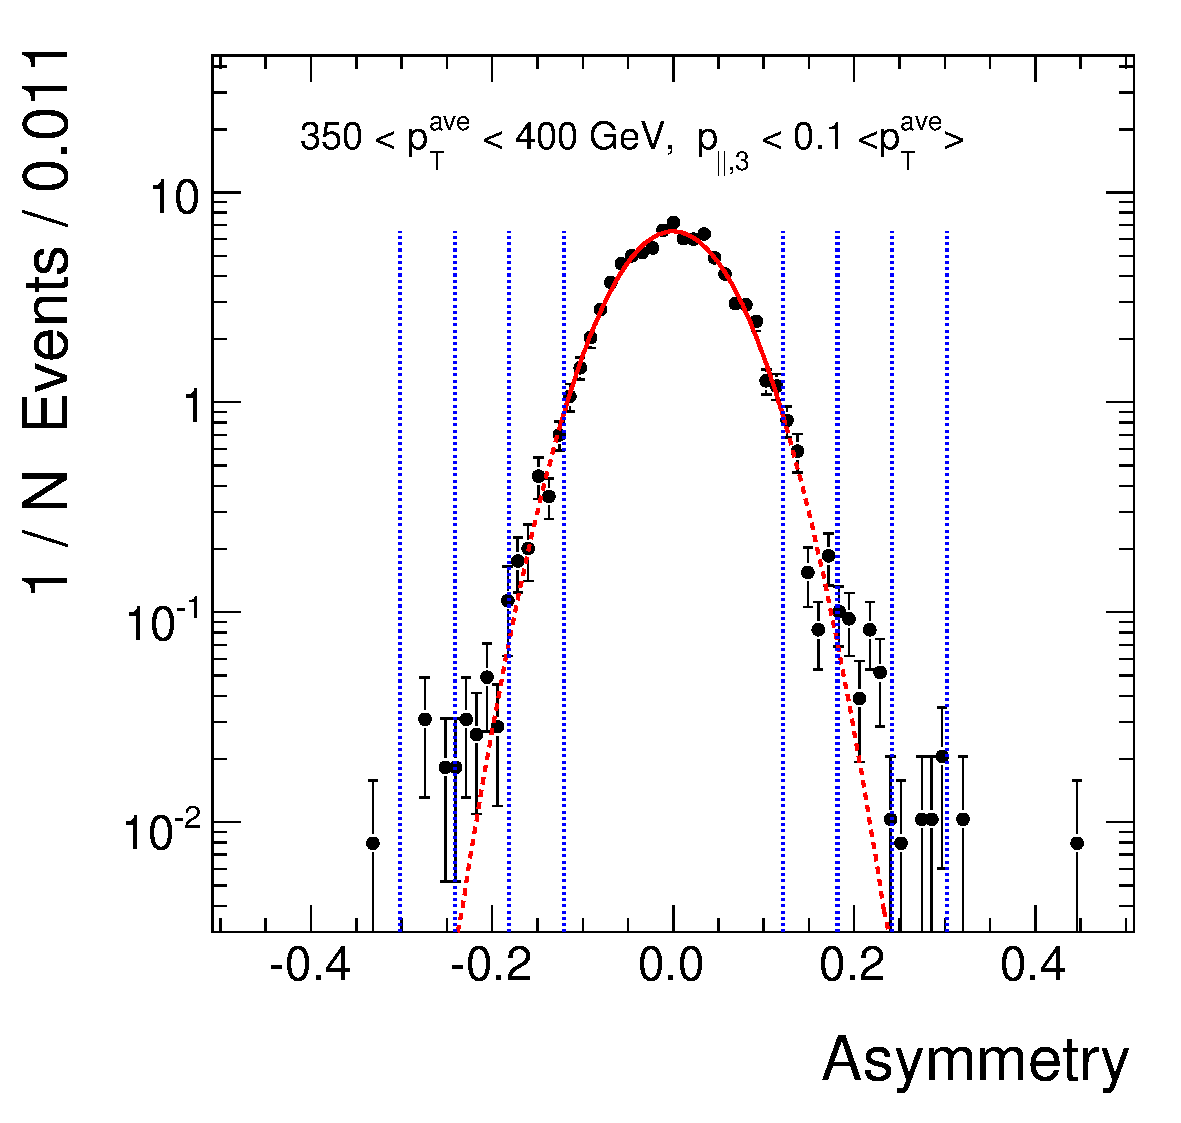
\includegraphics[width=0.45\textwidth]{figures/hTailsPtAsym} &
    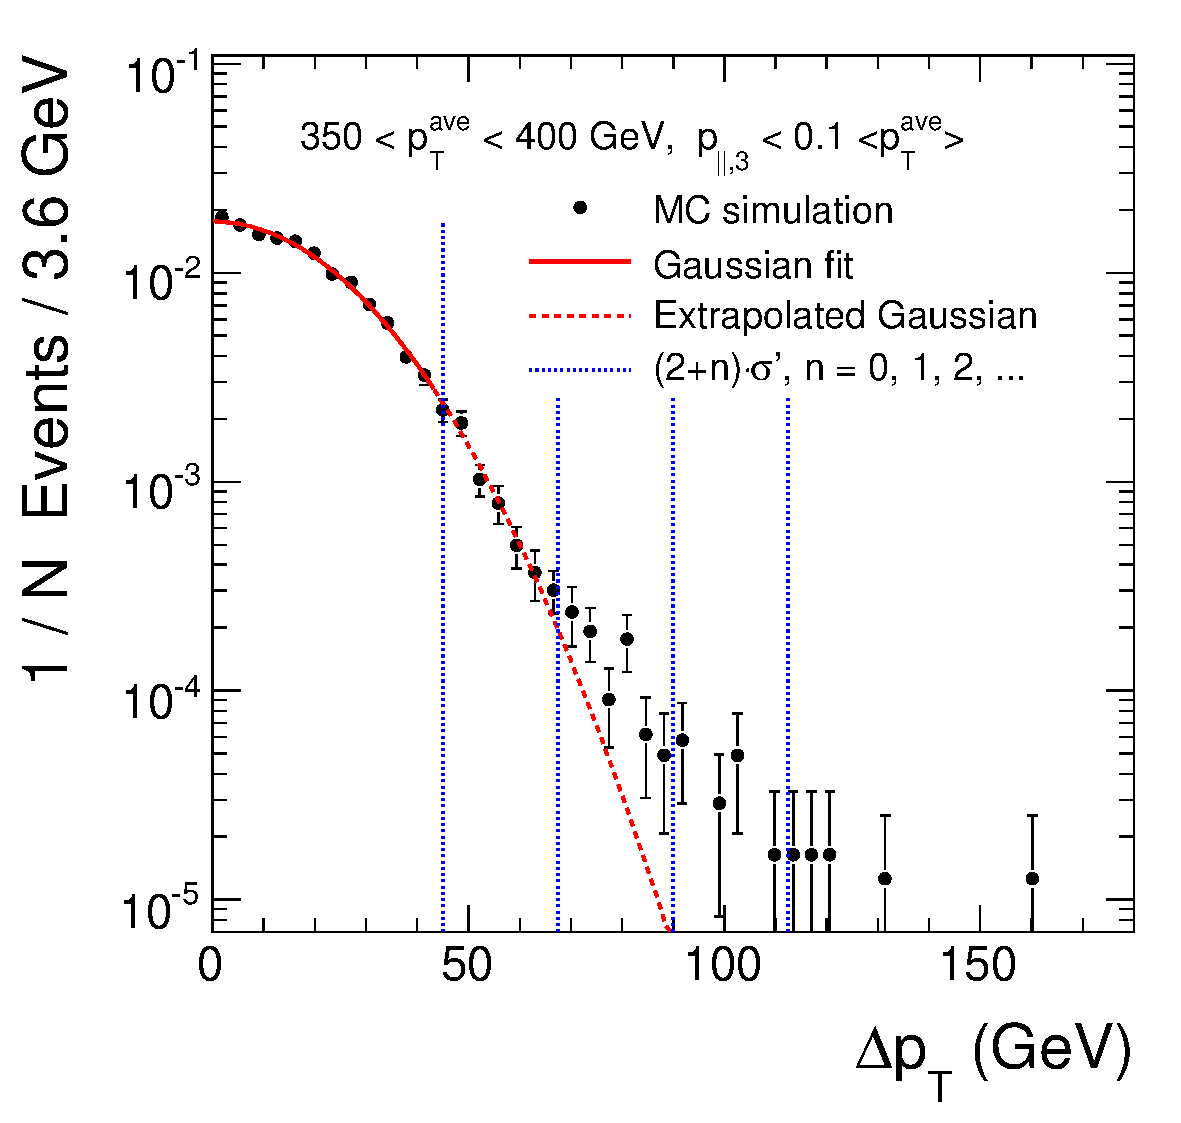
\includegraphics[width=0.45\textwidth]{figures/hTailsDeltaPt} \\
\end{tabular}
 \caption{Start of the non-Gaussian tails as expected from the MC simulation (circles) in the asymmetry (\textit{left}) and the corresponding \mbox{$\Delta\pt$} (\textit{right}) distribution.
   In each case, the central part of the distribution has been fitted with a Gaussian (solid line), which has been extrapolated further (dashed line) to guide the eye.
   Additionally, \mbox{$(2+n)\cdot\sigma'$} distances (dotted lines) are shown.}
  \label{fig:ResFit:DataDriven:Tails}
\end{figure}

\begin{figure}[ht]
 \centering
  \begin{tabular}{cc}
    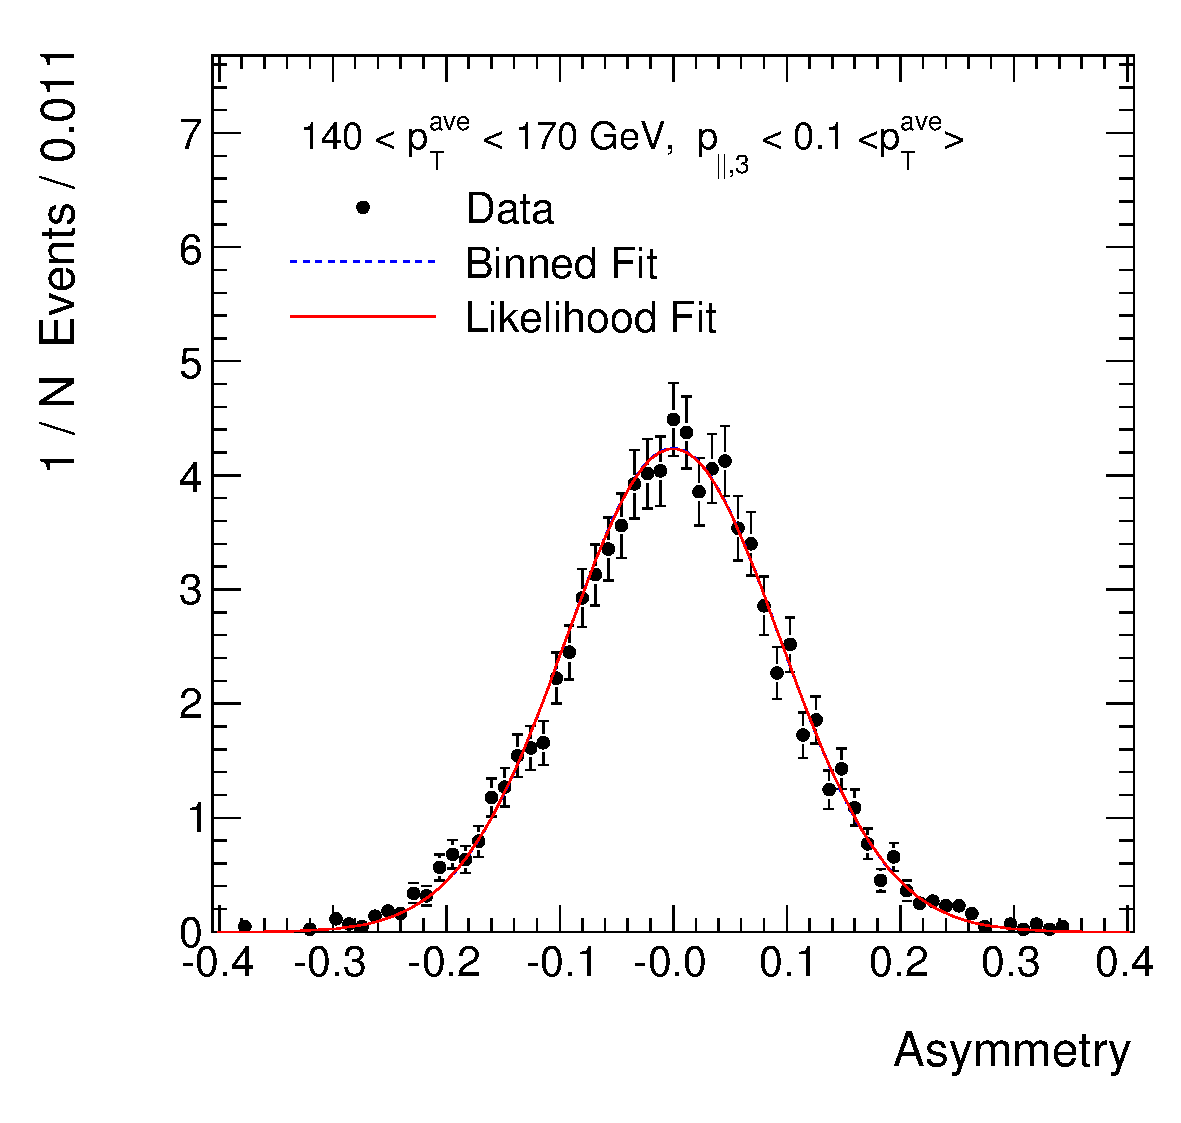
\includegraphics[width=0.45\textwidth]{figures/MaxLikeSimple_Data132440-144011_Eta00-13_PtAsymmetry_PtBin4_Pt3Cut3} &
    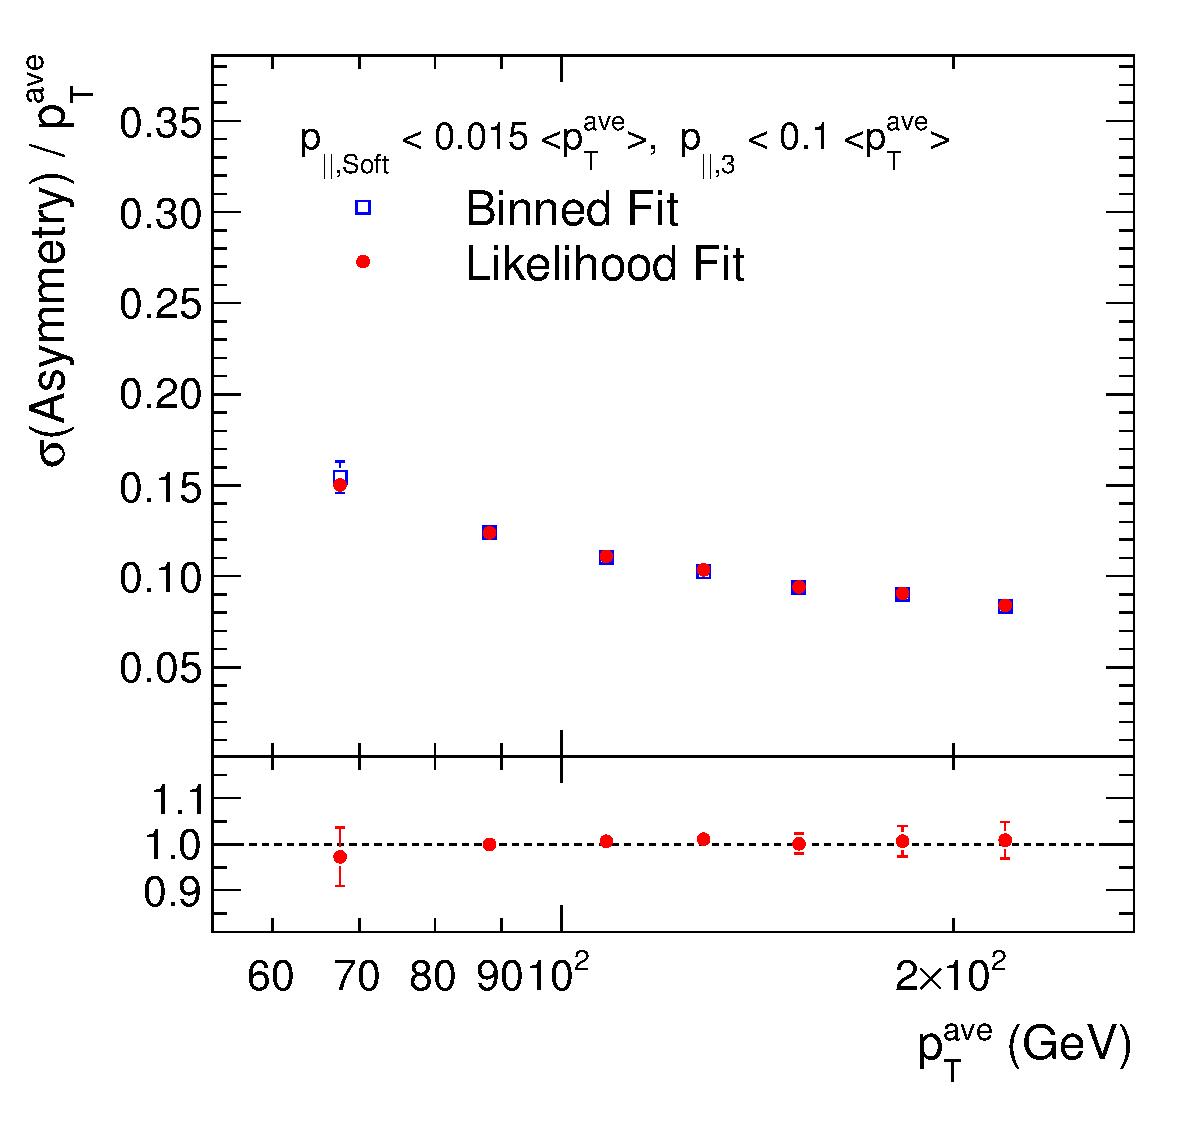
\includegraphics[width=0.45\textwidth]{figures/MaxLikeSimple_Data132440-144011_Eta00-13_PtAsymmetryWidthBottomRatio_Pt3Cut3} \\
\end{tabular}
 \caption{(\textit{Left}) Dijet asymmetry distribution measured in
    Collider data (solid circles) for \mbox{$140 < \ptave < 170\gev$}.
    It is well described by the prediction (solid line) from the
    simplified unbinned maximum likelihood fit and there is good agreement to a direct binned
    fit (dashed line) of the histogram.
    Note that both lines lie in fact on top of each other.
    (\textit{Right}) Gaussian widths of the asymmetry distributions in
    Collider data from binned fits of the
    histograms (open squares) in comparison to the results from
    the unbinned fit (solid circles) in different \ptave bins.}
  \label{fig:ResFit:DataDriven:Simple}
\end{figure}

However, in general there are non-Gaussian tails biasing the fit of the asymmetry.
In case of a binned fit of the histogram, the influence of the tails is suppressed by
fitting only the bulk of the distribution, defined as two standard deviations around the mean.
In case of the unbinned fit, it is not as straight forward to select only the bulk events.
This can be achieved, however, with an iterative procedure by restricting the allowed range of \mbox{$\Delta\pt$}.
As observed in the MC simulation (\qfig{fig:ResFit:DataDriven:Tails}), tails start to appear for \mbox{$|\Delta\pt| \gtrsim 3\sigma'$}.
(At this point, not enough Collider data has been analysed to measure the starting point of the tails.)
Hence, the unbinned fit is performed only for events with \mbox{$|\Delta\pt| < 2\sigma'$}; the tighter region is chosen to keep a safety margin in order to account for possible inaccuracies of the simulation.
Unitarity of the dijet pdf is preserved by adapting the normalisation of~\qeq{eq:ResFit::DijetPdfTransformed:Simple} accordingly.
(The complete pdf is given in~\qeq{eq:ResFit:App:SimplePdf} in Appendix~\ref{sec:ResFit:App:Pdf}.)

The threshold on $|\Delta\pt|$ in the above choice is proportional to $\sigma'$, which is the fitted parameter, and would be varied accordingly during the maximisation.
This, however, biases the result towards smaller values.
Therefore an iterative approach is chosen:
The threshold is kept fixed and the maximisation is performed leading
to a first estimate for $\sigma'$.
Then, the threshold is updated with this estimate and the maximisation is repeated.
This procedure is iterated four times, leading to an unbiased result.

The dijet asymmetry distribution measured in Collider data for \mbox{$140 <
  \ptave < 170\gev$} is shown in
\qsubfig{fig:ResFit:DataDriven:Simple}{left}.
Additional jet activity is suppressed by restricting their \pt components
along the dijet axis, \mbox{$\ppi{3} < 0.1\cdot\mean{\ptave}$} and
\mbox{$\ppi{\text{Soft}} < 0.015\cdot\mean{\ptave}$} (comp. \qsec{sec:ResFit:DataDriven:AddJets:Contributions} for
a definition of \pp).
It is well described by the result of the discussed simplified unbinned fit, \ie a Gaussian with width $\sigma'$, and there is good agreement to a direct binned fit of the histogram.
In \qsubfig{fig:ResFit:DataDriven:Simple}{right}, the widths $\sigma'$ measured in different \ptave bins with the unbinned technique are further compared to the results of binned fits.
Again, there is good agreement.

In conclusion, the simplified unbinned likelihood fit of the asymmetry performs equally to a binned fit of corresponding histogram.



\subsubsection{Full Maximum Likelihood Fit Including the Spectrum and Description of the Selection Bias}\label{sec:ResFit:DataDriven:FullFit}

In the following, the extension of the dijet pdf with an assumption for the particle level jet \pt cross section $f$ is discussed.
With the choice of coordinates~\qeq{eq:ResFit:TransformedCoordinates}, this corresponds to multiplying a pdf for the measured \ptave,
\begin{equation*}
 g_{\sigma'}\left(\ptave\right) \propto
  \int\dif{\pttrue}\;f\left(\pttrue\right)\cdot
  \e^{-\frac{1}{2}\left(\frac{\ptave - \pttrue}{\sigma'}\right)^{2}} \, , 
\end{equation*}
resulting in~\qeq{eq:ResFit:DijetPdfTransformed}.
As mentioned before, the spectrum is taken from the MC simulation (\qsubfig{fig:ResFit:DataDriven:Spectrum}{left}) and not modified during the fit.
The resulting systematic uncertainties are small, \qsec{sec:ResFit:Systematics}.

\begin{figure}[ht]
 \centering
  \begin{tabular}{cc}
    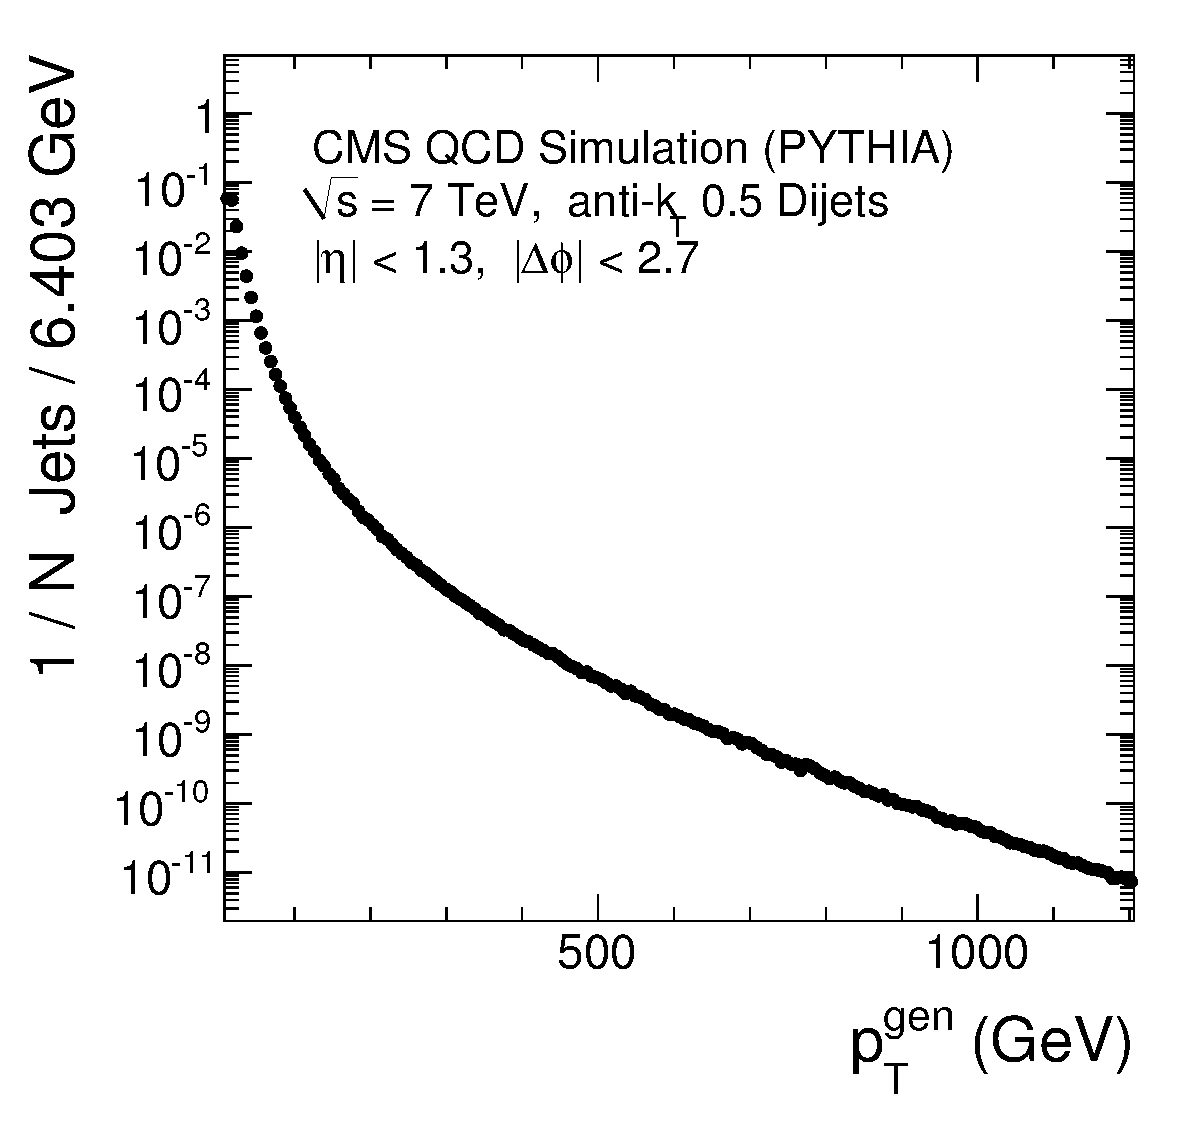
\includegraphics[width=0.45\textwidth]{figures/ExampleSpectrum} &
    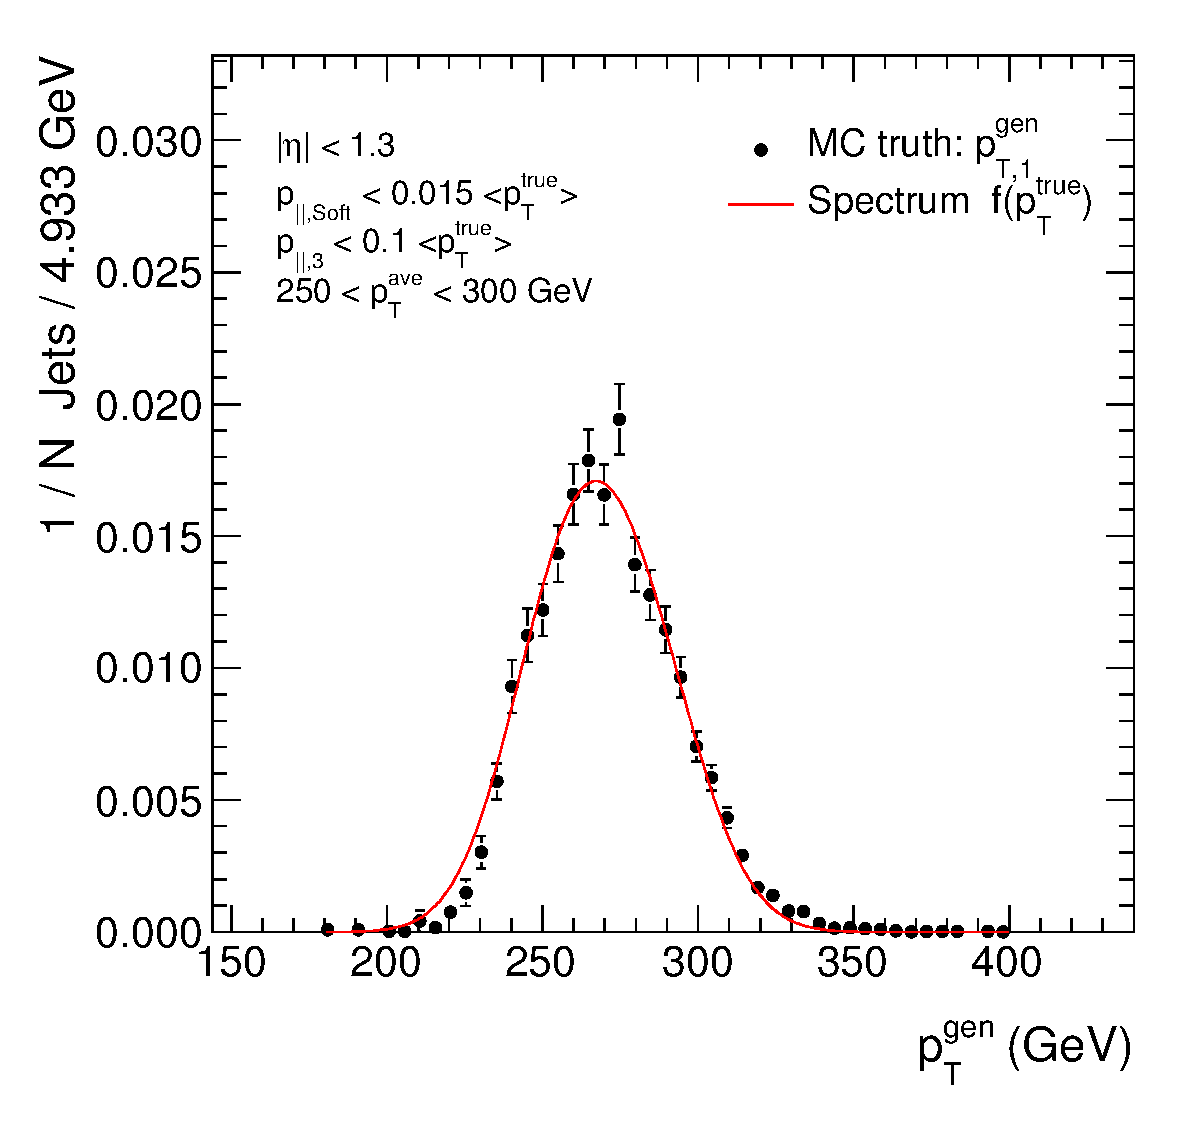
\includegraphics[width=0.45\textwidth]{figures/MaxLike_Eta00-13_SpectrumJet1_PtBin7}\\
 \end{tabular}
  \caption{(\textit{Left}) Dijet \ptgen spectrum from the MC simulation.
    Per selected event, the \ptgen of both the leading jets have been filled into the histogram.
    A linear interpolation of this histogram is used as the particle
    level differential jet cross section~ $f_{0}$ in~\qeq{eq:ResFit:DataDriven:ModifiedSpectrum}.
    (\textit{Right}) \ptgen spectrum (circles) of the selected dijet events in the \mbox{$250 < \ptave < 300\gev$} bin.
    It is well described by the modified cross section $f$ in~\qeq{eq:ResFit:DataDriven:ModifiedSpectrum} (line).}
  \label{fig:ResFit:DataDriven:Spectrum}
\end{figure}

By this extension, in addition a description of biases in the event selection can be included into the likelihood.
Binning in (measured) \ptave causes migration effects at the edges of the selected \ptave range due to the finite jet \pt resolution:
there are jets that fluctuate either into or out of the selected interval.
This is illustrated in \qsubfig{fig:ResFit:DataDriven:Spectrum}{right} with simulated data using the MC truth information.
Additionally, because of the steeply falling dijet \pt spectrum, in
any interval there are more jets that fluctuated high than jets that fluctuated low in \pt and the selected sample is therefore biased towards jets of lower \ptgen that fluctuated high in the detector.

The dijet pdf~\qeq{eq:ResFit:DijetPdfTransformed} is modified to describe the
\ptave selection and hence avoid biasing the measured resolution.
First, the allowed range of \ptave is considered in the normalisation (comp.~\qeq{eq:ResFit:App:FullPdf} in Appendix~\ref{sec:ResFit:App:Pdf}.)
Second, the \pttrue pdf is extended to incorporate the migration effects:
\begin{equation}
  \label{eq:ResFit:DataDriven:ModifiedSpectrum}
  f\left(\pttrue\right) = \frac{1}{\mathcal{N}_{f}}
  f_{0}\left(\pttrue\right) \int^{\ptavemax}_{\ptavemin}\dif{x}\;\mathcal{G}\left(x|\sigma',\pttrue\right) \, ,
\end{equation}
Here, $f_{0}$ denotes the underlying particle level jet \pt spectrum \qsubfig{fig:ResFit:DataDriven:Spectrum}{left}\footnote{The actual probability densities are evaluated using a linear interpolation of the histogram.} and $\mathcal{G}$ is a Gaussian of width \mbox{$\sigma' = \sigma/\sqrt{2}$}, \ie the pdf of \ptave for a given \pttrue.
Equation~\qeq{eq:ResFit:DataDriven:ModifiedSpectrum} is validated using simulate data:
the \ptgen spectrum of selected dijet events is well described by $f(\pttrue)$ as demonstrated in \qsubfig{fig:ResFit:DataDriven:Spectrum}{right}.
This extension to $f$ depends solely on the fitted parameter $\sigma'$ and does not introduce any new dependencies on the MC simulation.



\subsection{Influence of Additional Hadronic Activity and Hadronisation Effects}\label{sec:ResFit:DataDriven:AddJets}

\subsubsection{Contributions to the Dijet Asymmetry}\label{sec:ResFit:DataDriven:AddJets:Contributions}

In \qsubfig{fig:ResFit:DataDriven:AddJets:Bias}{right}, the standard deviations of
the asymmetry distribution, multiplied by a factor $\sqrt{2}$,
are shown for various \ptgen bins for simulated dijets.
According to~\qeq{eq:ResFit:ResFromAsym} these should correspond to the
jet \pt resolution.
However, they are greater than the MC truth resolutions\footnote{The
  determination of the MC truth resolution is discussed in
  Appendix~\ref{sec:ResFit:App:MCTruth}.} $\sigma(R_{\text{MC}})$ for
the following reasons:
The dijet asymmetry~\qeq{eq:ResFit:Asymmetry} is defined under the assumption of exactly two jets which are balanced in transverse momentum at particle level.
Additional jet activity in the events, \eg from soft gluon
radiation, causes an imbalance of the leading two jets and hence
broadens the measured asymmetry distribution.

\begin{figure}[ht]
 \centering
  \begin{tabular}{cc}
    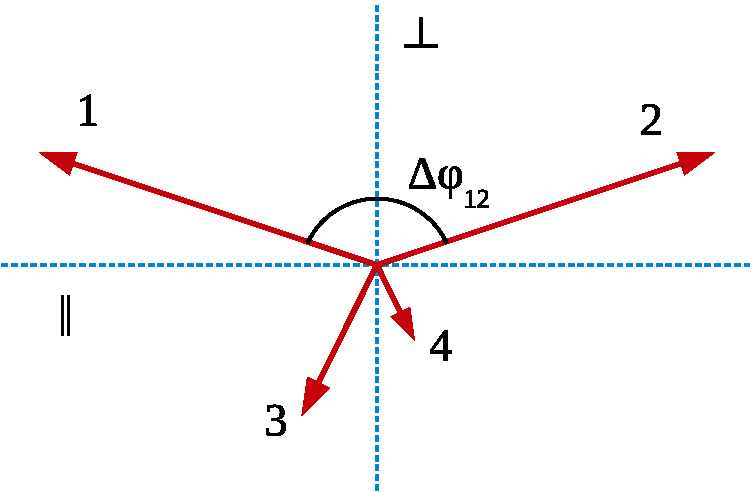
\includegraphics[width=0.45\textwidth]{figures/Sketch_Projections} &
    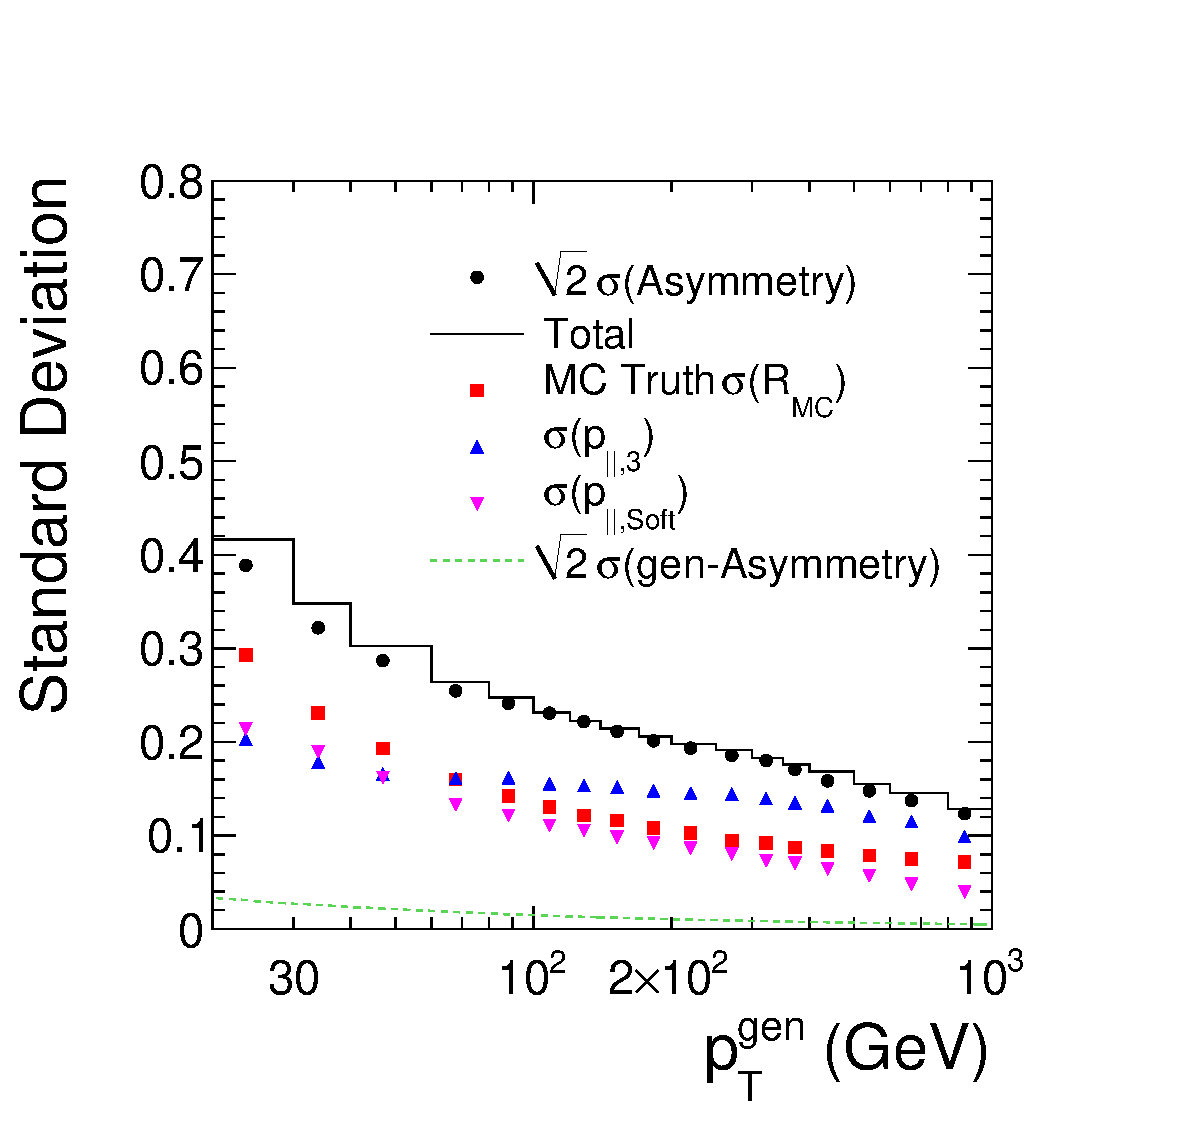
\includegraphics[width=0.45\textwidth]{figures/Spring10QCDDiJet_ParallelComponent_hParallelContributions} \\
 \end{tabular}
  \caption{(\textit{Left}) Definition of the dijet axis $\phi_{||}$, the direction normal to the
    angle bisector of the leading two jets in the transverse plane.
    Additional jets with \pt components along $\phi_{||}$ will cause
    a \pt imbalance of the particle jets and bias the measured
    resolution towards greater values. 
    (\textit{Right}) Demonstration of the different
    contributions biasing the measured dijet asymmetry and hence resolution.
    Shown are the standard deviations of the distributions of the
    different quantities described in the text. 
    Their quadratic sum (solid line) is in fair agreement to the
    measured asymmetry (solid circles).
    For this plot, simulated dijet events have been preselected by requiring \mbox{$|\Delta\phi_{12}| > 2.7$}.
 }
  \label{fig:ResFit:DataDriven:AddJets:Bias}
\end{figure}

As illustrated in \qsubfig{fig:ResFit:DataDriven:AddJets:Bias}{left}, not the
absolute \pt of the additional jets actually affects the balance, but rather the component along the dijet axis, $\phi_{||}$, defined as the direction normal to the angle bisector of the leading two jets.
The \pt components parallel to $\phi_{||}$ of the third and all further
(\textit{soft}) jets may be defined as
\begin{align}
  \begin{split}
    \ppi{3}               & =  |\pti{3}\cos(\phi_{3}-\phi_{||})| \\
    \ppi{\text{Soft}} & =  |\sum_{i>3}\pti{i}\cos(\phi_{i}-\phi_{||})| \,.
  \end{split}
\end{align}
The total standard deviation of the measured dijet asymmetry
distribution (multiplied by $\sqrt{2}$) can hence be understood as the
quadratic sum of the underlying dijet asymmetry due to the jet \pt response,
$\sigma(R_{\text{MC}})$, and the standard deviations of the \pp
distributions, $\sigma(\ppi{3})$ and
$\sigma(\ppi{\text{Soft}})$,
\begin{equation}
  \label{eq:ResFit:TotalAsym}
  \text{Total} = \sigma(R_{\text{MC}}) \oplus \sigma(\ppi{3}) \oplus
  \sigma(\ppi{\text{Soft}}) \oplus \sqrt{2}\cdot\sigma(A^{\text{gen}}) \,.
\end{equation}

The transverse momentum balance assumed for the particle level jets
actually takes place at parton level.
Due to the statistical nature of the fragmentation and hadronisation
process, fluctuations in the
fraction of energy of the original partons clustered into jets are
expected (\textit{out-of-cone}).
This is an additional mechanism introducing an imbalance in the
dijet events and the contribution is estimated using the \ptgen
asymmetry, $A^{\text{gen}}$, in perfect
two jet events.
The standard deviation $\sqrt{2}\cdot\sigma(A^{\text{gen}})$ is also added in quadrature to
$\sigma(R_{\text{MC}})$, hence the last term in~\qeq{eq:ResFit:TotalAsym}.

The dijet pdf~\qeq{eq:ResFit:DijetPdf} has been shown to be a pdf of
the dijet asymmetry and has also been defined under the assumption of \pt
balance at particle level.
Hence it will be biased by the same effects.



\subsubsection{Correction for Additional Hadronic Activity}\label{sec:ResFit:DataDriven:AddJets:Extrapolation}

In order to compensate for the presence of additional jets,
events are selected\footnote{The resulting selection bias is incorporated in the dijet pdf as
before, comp. \qsec{sec:ResFit:DataDriven:FullFit}.} in reasonably small bins of \ptave.
Per bin, the \pp components of the third and all further jets are restricted to
\begin{align}
  \label{eq:ResFit:ThirdJetSelection}
  \begin{split}
    \ppi{3}                & < z\cdot\mean{\pttrue} \\
    \ppi{\text{Soft}}  & < 0.015\cdot\mean{\pttrue},
 \end{split}
\end{align}
where $\mean{\pttrue}$ is the mean particle level jet \pt in that bin
as estimated from the assumed spectrum
$f$ in~\qeq{eq:ResFit:DataDriven:ModifiedSpectrum}.
Several sets of dijet events are selected, each with a different
threshold $z$ of \ppi{3}, and the mean Gaussian response with \pt
independent resolution $\sigma$ is measured by maximising the dijet
likelihood~\qeq{eq:ResFit:Likelihood} w.r.t. $\sigma$.
The dependence of the jet \pt resolution on the threshold $z$ is
clearly visible in \qfig{fig:ResFit:DataDriven:AddJets:Corr}.
In order to extrapolate the measurement to the case of a two jet only
event, the \mbox{$\sigma/\mean{\pttrue}$} are fitted with a linear
function and the $y$ axis intercept is used as the unbiased jet \pt
resolution.

\begin{figure}[ht]
 \centering
 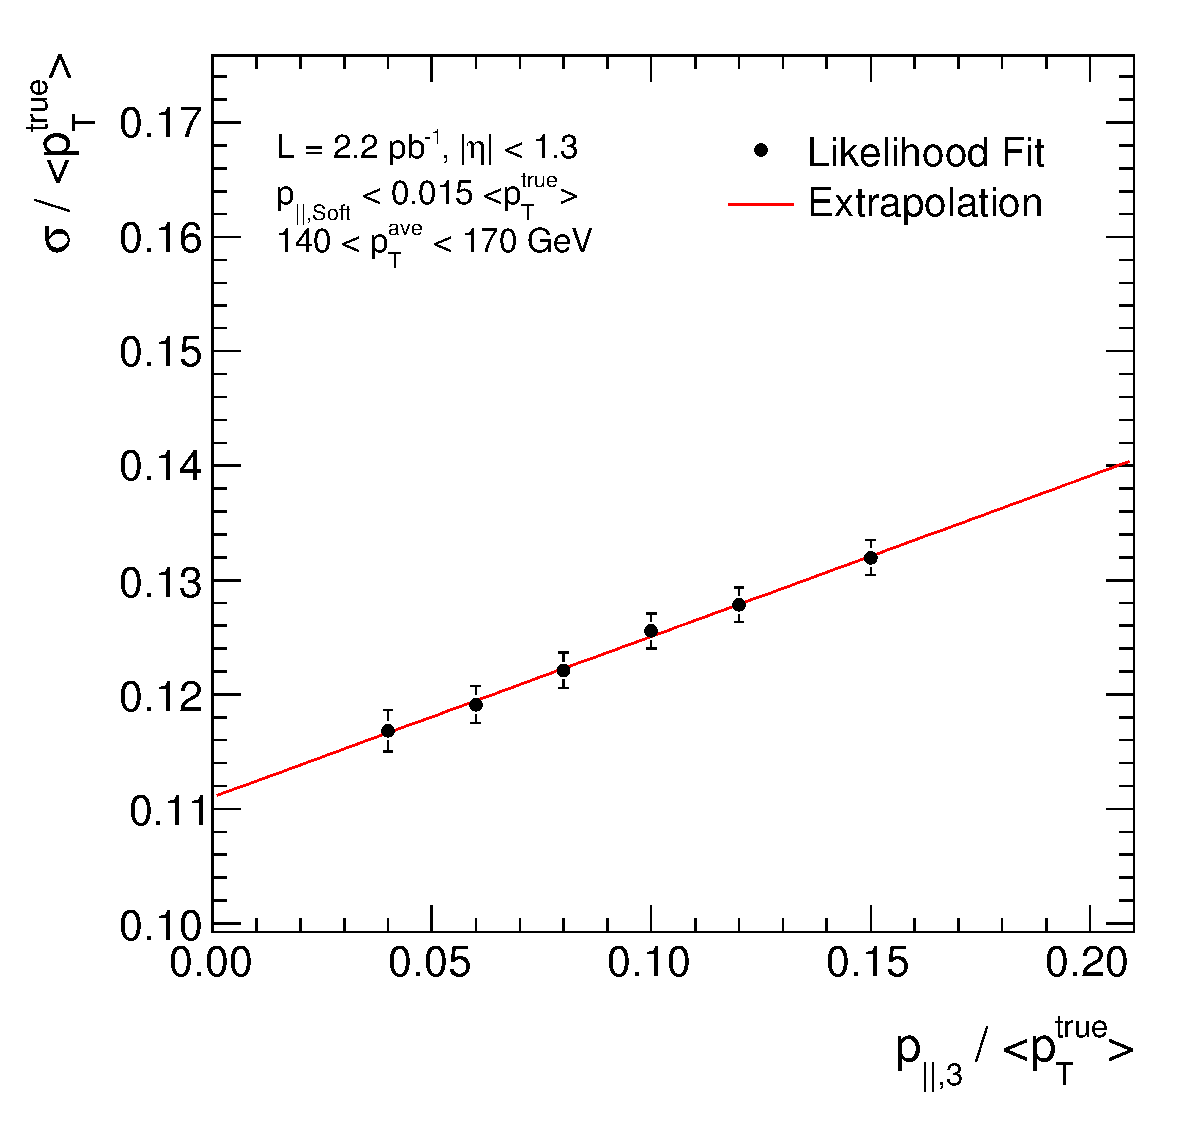
\includegraphics[width=0.45\textwidth]{figures/MaxLike_Data132440-144011_Eta00-13_ExtrapolatedPar0_PtBin4}
 \caption{(\textit{Right}) Gaussian resolutions \mbox{$\sigma/\mean{\pttrue}$} measured with the unbinned
    fit in Collider data for \mbox{$140 < \ptave < 170\gev$} and different \ppi{3}
    thresholds after suppression of additional soft jet activity along
    $\phi_{||}$. 
    \mbox{$\sigma/\mean{\pttrue}$} of \ppi{3} is linearly
    extrapolated to the case of an ideal dijet event.
  }
  \label{fig:ResFit:DataDriven:AddJets:Corr}
\end{figure}

In the following, the statistical uncertainty on the fitted $y$ axis
intercept is used as statistical uncertainty of the measured resolution.
Due to the selection requirement~\qeq{eq:ResFit:ThirdJetSelection},
all events selected for a particular value of the threshold $z$ are
also included in the samples selected with larger values of $z$.
Hence, the measured resolutions in one \ptave bin are strongly correlated.
This correlation is not considered in the quoted uncertainties yet.

The contribution due to out-of-cone effects to the bias is small, of
the order of $1\%$, as shown in
\qsubfig{fig:ResFit:DataDriven:AddJets:Bias}{right}.
Hence, this bias is corrected for using the MC simulation:
The width of the \ptgen asymmetry, $\sigma(A^{\text{gen}})$, is determined for the
 case of perfectly balanced dijet events, using the
same extrapolation technique as above.
The extrapolated jet \pt resolution is then corrected by 
subtracting $\sqrt{2}\cdot\sigma(A^{\text{gen}})$ in quadrature.

The need for compensating the influence of additional jet activity is
the reason why a mean, \pt independent resolution is
measured per \ptave bin.
In that case, there is only one free parameter, $\sigma$, which can be
extrapolated in a straight forward way.
If the response is instead parameterised with a \pt dependent function,
\eg a Gaussian with width \mbox{$\sigma(\pt) = a\pt \oplus
  b\sqrt{\pt} \oplus c$},
the parameters $a$, $b$, and $c$ are correlated.
The method of the maximum likelihood fit itself is not affected by the
parameter correlation, however, and can very well measure the
parameters of a \pt dependent resolution $\sigma(\pt)$ as demonstrated
in Appendix~\ref{sec:ResFit:App:ToyMC} using a toy MC simulation.

